\documentclass[twocolumn, a4paper]{ieicejsp}
%\usepackage{newenum}
%\usepackage[dvipdfmx]{graphicx}
\usepackage{epsfig}
\usepackage[fleqn]{amsmath}
\usepackage{amssymb}
\usepackage{comment}
%\usepackage{textcomp}
%\usepackage{lmodern}
%\usepackage{mediabb}

\setcounter{topnumber}{5}%    ページ上部の図表は 5 個まで
\def\topfraction{1.00}%       ページの上 1.00 まで図表で占めて可
\setcounter{bottomnumber}{5}% ページ下部の図表は 5 個まで
\def\bottomfraction{1.00}%    ページの下 1.00 まで図表で占めて可
\setcounter{totalnumber}{10}% ページあたりの図表は 10 個まで
\def\textfraction{0.04}%      ページうち本文が占める割合の下限
%        これを 0 にすると本文が 1 行だけのページが出来る
%        0.04 くらいにすると 1 行だけのページは防げる
%        0.1 くらいが良いかも知れない
\def\floatpagefraction{0.7}%  図表だけのページは少なくとも
                           %  これだけを図表が占める

\title{
{\bf 全二重通信無線LANにおける公平性を考慮した\\端末組み合わせの検討}
{\normalsize \\Station Pairing Considering fairness for In-Band Full-Duplex Wireless LANs}
}

\author{
{飯田直人$^1$} \\ {N. Iida} \and
{西尾理志$^1$} \\ {T. Nishio} \and
{守倉正博$^1$} \\ {M. Morikura} \and
{山本高至$^1$} \\ {K. Yamamoto} \and
{鍋谷寿久$^2$} \\ {T. Nabetani} \and
{青木亜秀$^2$} \\ {T. Aoki}
}

\affliate{
{\small 京都大学大学院情報学研究科$^1$}\\
{\small Graduate School of Informatics, Kyoto University}\\
\and
{\small 東芝 研究開発センター$^2$}\\
{\small Corporate Research \& Development Center, TOSHIBA Corporation}
}

\renewcommand{\baselinestretch}{0.85}\selectfont %0.6まで大丈夫

\begin{document}
%\setlength{\abovedisplayskip}{5pt} % 上部のマージン
%\setlength{\belowdisplayskip}{5pt} % 下部のマージン
\maketitle
\section{はじめに}
全二重通信無線LANでは送信と受信を同時に同じ周波数帯で行うため,自己干渉と端末間干渉が問題となる.
既に最適化問題を用いて,これらの干渉を考慮した上で全二重通信を行う端末(STA)の組み合わせを確率的に決定するMACプロトコル~\cite{promac}が検討されている.
しかし,~\cite{promac}は干渉の少ないSTAの組み合わせが選ばれやすく,
STA間の送信機会に関する公平性が低下する問題がある.
本稿では,各STAの待機時間を考慮することで,送信機会の公平性を向上する.

\section{システムモデル\label{モデル}}
100\,m四方の領域の中心に1台のアクセスポイント(AP)が存在し,
50台のSTA(STA 1,..., STA 50)がランダムに配置されている状況を考える.
50台のSTAの中から,APからの下り通信を受信するSTA $i$とAPへの上り通信を行うSTA $j$の組み合わせを最適化問題を用いて確率的に決定する.
このとき,STAの組み合わせを$(i,j)$と表現し,$i, j = 0, 1, 2,...,50$であり,$i\neq j$とする.
ただし,$i=0$のときは上り通信のみの半二重通信,$j=0$のときは下り通信のみの半二重通信を表すものとする.

\section{最適化問題の設計 \label{方法}}
本稿で検討する最適化問題は以下のとおりである.
\begin{align}
	&{\mathcal P}_1: && {\rm max} \sum_{(i,j)\in{\mathcal C}} p^{(i,j)}r^{(i,j)}(d^{(j)})^{\alpha} &&&&&& \\
	&{\rm subject\ to} && \sum_{j\in\{j:(i,j)\in{\mathcal C}\}} p^{(i,j)} \geq \eta_{\rm d}^{(i)}, \forall i\in {\mathcal N}  \\
	&&& \sum_{i\in\{i:(i,j)\in{\mathcal C}\}} p^{(i,j)} \geq \eta_{\rm u}^{(j)}, \forall j\in {\mathcal N}  \\
	&&& \sum_{j\in\{j:(i,j)\in{\mathcal C}\}} p^{(i,j)}=1 \\
	&{\rm variables:} && p^{(i,j)} \in {\mathbb R}_{\geq 0},\forall(i,j)\in {\mathcal C}
\end{align}
$p^{(i,j)}$は$(i,j)$の組み合わせで通信が行われる確率,
$r^{(i,j)}$はその組み合わせで通信が行われた場合の上下の推定スループットの和,
$d^{(j)}$はSTA $j$のバッファの先頭にあるフレームの先頭に来てからの待機時間,
$\alpha$は重み付けのためのパラメータ,
$\eta_{\rm d}^{(i)}$はSTA $i$への下り通信のトラヒック量に比例した値,
$\eta_{\rm u}^{(j)}$はSTA $j$のAPへの上り通信のトラヒック量に比例した値,
${\mathcal N} = \{1,2,...,50\}$,
${\mathcal C}$は組み合わせの集合である.
APは$p_{\rm d}^{(i)}=\sum_{j\in\{j:(i,j)\in{\mathcal C}\}}p^{(i,j)}$で得られる確率をもとにSTA $i$を選択し,STA $j$は確率$p_{\rm u}^{(i,j)}=p^{(i,j)}/p_{\rm d}^{(i)}$の逆数をウィンドウサイズとしたバックオフアルゴリズムによって送信権を獲得する.
\par
従来研究~\cite{promac}では,評価関数には確率$p^{(i,j)}$と推定スループット$r^{(i,j)}$のみが含まれており,
$r^{(i,j)}$が大きい,つまり,干渉が少ないSTAの組み合わせが選択される確率が高くなる.
本稿では,評価関数に待機時間$d^{(j)}$の項を加えることで,待機時間が大きいSTAの送信確率が高くなるよう設計し,
上り通信の送信機会の公平性を改善することを可能とする.
また,重み付けの$\alpha$を用いることで,待機時間が最適化の結果に与える影響を調整し,
システムの要求に応じて,システムスループットと送信機会の公平性のバランスを調整することができる.

\section{シミュレーション評価 \label{評価}}
前述の最適化問題を用いた端末選択によって,送信機会の公平性が改善することを確かめる.
また,$\alpha$の調整によるシステムスループットと公平性のバランスの変化を示す.
公平性の評価にはJain's fairness index~\cite{fair}を用いる.
伝送速度にはシャノン容量を用い,公平性の評価には各STAの送信回数を用いている.
結果は10トポロジーの平均である.
\par
図\ref{fig:thr_fair}に$\alpha$に対するシステムスループット,STAの送信機会の公平性を示す.
$\alpha=0$のときが待機時間を考慮しない場合~\cite{promac}に相当し,それに比べ$\alpha>0$とし,待機時間を考慮すると大きく公平性が改善することがわかる.
それと引き換えに$\alpha$が大きいとシステムスループットが減少していることが確認できる.

\begin{figure}[t]
	\centering
	\epsfig{file=../graph/thr_fair.eps, scale=0.5}
	\caption{重み$\alpha$に対するシステムスループットと公平性}
	\label{fig:thr_fair}
\end{figure}

\section{まとめ}
本稿では,全二重通信無線LANにおいて干渉を考慮した上での送信機会の公平性改善について検討した.
シミュレーションの結果,評価関数に待機時間の項を加えることで公平性を改善できることを示した.
さらに,待機時間の重みを変化させることで,システムスループットと公平性のバランスを調整できることを示した.


\small
\bibliographystyle{ieice}
\begin{thebibliography}{9}
\bibitem{promac} S. Y. Chenn et al.,``Probabilistic-based adaptive full-duplex and half-duplex medium access Control,'' IEEE GLOBECOM,  pp 1-6, Dec. 2015.
\bibitem{fair} R. Jain et al.,``A quantitative measure of fairness and discrimination for resource allocation in shared computer system,'' DEC Technical Report 301, 1984.
\end{thebibliography}
\end{document}
